
\section{Experiments}

In this section, we describe our experimental evaluation of the
performance of the PC distributed computation system for a set of
representative big data analytics problems. The aim is to answer
following questions:

\begin {enumerate}
\item How useful is PC in building tools and libraries for big data analytics?
\item How efficient and easy is PC in manipulating highly nested and complex objects?
\item How well is PC in performing complex computations like real
  machine learning applications?
\end {enumerate}

\subsection {Experimental Environment and Applications}

All of the experiments reported in this paper were performed in a
cluster that consists of eleven Amazon EC2 m2.4xlarge machines,
running Ubuntu 16.04. Each machine had eight virtual cores, one SSD
disk, and 68 GB of RAM). One of the eleven machines served as the Master
node and the rest ten machines served as Worker nodes.

\vspace{5pt}
To conduct convincing benchmarks and performance comparisons, we
selected eight representative applications from three categories
of big data analytics workloads that are important for demonstrating
PC's utilities and performance:

\begin {itemize}
\item \texttt{Linear Algebra Library.} We constructed a linear algebra library
  and tested three common linear algebra computations: Gram Matrix,
  Linear Regression, and Nearest Neighbor Search.
\item \texttt{Analytical queries on TPC-H Data
    Set.}  We implemented two typical analytical queries against TPC-H
  benchmark data set that were denomalized to complex nested objects: the first one is an aggregation query reporting which customer buys which
  parts for each supplier; the second one is a Top-K similarity query
  to search for K customers who buy the closest items compared with a
  given customer.
\item \texttt{Machine Learning.} We also implemented three widely used
  iterative and complex machine learning algorithms: \textbf{Latent Dirichlet Allocation (LDA)}--A
  generative statistic model for text topic mining;
  \textbf{Gaussian Mixture Model (GMM)}--A clustering algorithm to generate a composite
  distribution whereby points are drawn from one of multiple Gaussian distributions;  and \textbf{KMeans}-- A well-known clustering algorithm that clusters
  data points into a pre-defined number of clusters.
\end {itemize}





\subsection {Construction of a distributed linear algebra library}
Since PC is designed to support the construction
of high-performance tools and libraries, our first benchmarking effort was aimed at determining 
whether PC is actually useful for that task.  Thus, we asked
a graduate student who knew nothing of PC to use the system to build a small Matlab-like 
programming language and library for distributed matrix operations.
We called this implementation \texttt{LilLinAlg}.

Our goal was to determine the 
performance and functionality that an expert programmer (but PC novice) could deliver in a short
timeframe, compared to a set of established distributed Big Data matrix implementations:
SciDB \cite{brown2010overview, stonebraker2011architecture} (built from the ground up by an MIT team over the last nine years), MLLib \cite{meng2016mllib} 
(the Big Data matrix
implementation shipped with Spark), and SystemML \cite{boehm2014hybrid, ghoting2011systemml, boehm2016systemml}
(a matrix and machine learning implementation developed
over the last seven years by a team at IBM, built on top of Spark and Hadoop).
The student spent about six weeks in this effort.

\subsubsection {Implementations}
In \texttt{LilLinAlg}, a distributed matrix is a PC dataset of dense matrix
blocks that is backed by one or more pages which can be buffered/cached in PC's distributed buffer pool and
persisted to PC's distributed user-level file system. Each dense matrix
block in the PC dataset is encapsulated as a MatrixBlock object that contains a
Vector of doubles and meta data that specifies the row and column
dimensions of this matrix block. All MatrixBlock in one distributed
matrix Set have equivalent row and column dimensions that can be
specified when a user claims a new distributed matrix dataset. A
MatrixBlock should be small enough to fit to a page (by default, page size
is 256 mega bytes).

\texttt{LilLinAlg} implemented common distributed matrix
computations on top of the PC platform, including $transpose$,
$inverse$, $add$, $substract$, $multiply$, $transposeMultiply$, $scaleMultiply$, $MinElement$,
$MaxElement$, $RowSum$, $ColumnSum$, $DuplicateRow$, $DuplicateCol$
and many more. Each computation can be translated to a partial PC query
graph. Taking $multiply$ for example, it will be translated to a partial
PC query graph that consists of a join and an aggregation like following:

\begin{code}
Handle <Computation> query1 = makeObject <LAMultiplyJoin> ();
query1->setInput (0, leftChild->evaluate(instance));
query1->setInput (1, rightChild->evaluate(instance));
Handle <Computation> query2 = makeObject <LAMultiplyAggregate> ();
query2->setInput(query1);
\end{code}

Here, the LAMultiplyJoin and LAMultiplyAggregate are both user-defined Computation classes that are
derived from the JoinComp class and AggregateComp class, which are
part of PC's declarative interface,  respectively. \texttt{LilLinAlg}
implemented the distributed matrix multiplication logic manipulating
two distributed matrixes (each is a dataset consists multiple
MatrixBlock objects that can be distributed across the cluster) through these
two user-defined classes. The LAMultiplyJoin
and LAMultiplyAggregate invoke numerical processing libraries such as
Eigen to manipulate MatrixBlock objects. Because each
MatrixBlock is backed by a Vector<double> Object, the pointer to the
raw array data is directly passed to Eigen library for efficient processing.

\texttt{LilLinAlg} also provided a linear algebra DSL for user to
easily express the linear algebra tasks in mathematical language. For
example, a least squares linear regression task can be easily coded as
\texttt{X = load(myMatrix.data); beta = (X '* X)\^{}-1 \%*\% (X '*
  y)}. 
In above DSL expression, \texttt{'*} represents a transposeMultiply computation,
\texttt{\^{}-1} represents an inverse computation, and \texttt{ \%*\%}
represents a multiply computation. 

\texttt{LilLinAlg} contained a compiler
to automatically translate the user program like above into a PC query graph that
connects (and optimizes) the partial PC query graphs corresponding to
each compuation to form the final query graph. Then it submits the
final query graph to the underlying PC platform for execution. 

In PC, the query
graph is automatically compiled to TCAP, which is then analyzed, optimized and compiled to native
code that gets executed in the PC distributed framework.

The \texttt{LilLinAlg} package consists of 3500+ lines of C++ code,
2700+ lines of C code that is automatically generated by yacc/lex, 
plus a few yacc/lex code.

\subsubsection {Experiments}

We ran three different computations:
a Gram matrix computation (given a matrix $\textbf{X}$, compute
$\textbf{X}^T \textbf{X}$), least squares linear regression (given a matrix of features $\textbf{X}$ and
responses $\textbf{y}$, compute 
$\hat{\pmb{\beta}} = (\textbf{X}^{T} \textbf{X})^{-1} \textbf{X}^{T} \textbf{y}$), and nearest
neighbor search in a Riemannian metric space \cite{lebanon2006metric} encoded by matrix $\textbf{A}$ (that is,
given a query vector
$\textbf{x}'$ and matrix $\textbf{X}$, find the $k$ rows in the matrix that minimize 
$d_{\textbf{A}}^2(\textbf{x}_i, \textbf{x}') = 
(\textbf{x}_i - \textbf{x}')^T\textbf{A}(\textbf{x}_i - \textbf{x}')$).  All experiments used
ten Amazon
EC2 m2.4xlarge workers.  

For Gram matrix and linear regression, SystemML V0.9 on Hadoop,
and Spark 1.6.1 was used; for
nearest neighbor, SystemML V1.0 on Spark and Spark 2.1.0 was used. We
use the same SciDB version 14.8 for all three
experiments.

For experiments on the PC platform, we mainly tuned the page size of the
distributed matrix dataset for different dimensions to make sure the
matrix can be fully distributed across the cluster:
we use 4 mega bytes page size for 10 dimensions, 16 mega bytes page
size for 100 dimensions, and 64 mega bytes for 1000 dimensions. In addition, PC's query optimizer dynamically decided to use
broadcast join when one input dataset of the join is smaller than two
giga bytes, and to use hash partition join when both input datasets of
the join is larger than two giga bytes.

For experiments on other platforms, we also carefully tuned the
systems for best performance. For example, we tuned Spark block size and repartition
size for every experiment. In SystemML, we also carefully chose to
use the parallel for loop, which boost performance significantly.

For
all three computations, 
$10^6$ data points were used. For each computation, 10, 100 and 1000
dimensions are tested.


\subsubsection {Results}

Results are given in 
Table \ref{fig:LR}. It shows for the most complex task, the nearest
neighbor computation, for both 100 and 1000 dimensions, PC
\texttt{LilLinAlg} provided the best performance compared with latest
SystemML, Spark and SciDB. It achieved $1.5\times$ speedup compared with
the next winner, the Spark-based
SystemML V1.0 with the latest version. For 10 dimension, PC performs slower
than SystemML, because SystemML runs small computation in local
mode. PC also achieved more than $10\times$ speedup compared with
Spark version 2.1.0, and $6\times$ speedup compared with SciDB version
14.8. 

For Gram Matrix and Linear Regression with high dimensions, PC achieved up to
$4\times$ speedup compared with the the Hadoop-based SystemML V0.9, up to $27\times$
speedup compared with Spark version 1.6.0, and up to $5\times$ speedup compared
with SciDB version 14.8.

We need point out that, although SystemML and Spark MLLib are
Java/Scala based, for their versions used
in all experiments, native
numerical librarires such as OpenBLAS are installed and invoked, so as to
the computation tasks, there is not much lanugage advantages that can
be taken by PC. Most performance benefits are from reduced
serialization/deserialization time with the PC object model, TCAP optimization and PC
backend's relational syle of processing objects.


\begin{table}[h!]
\begin{center}
\begin{tabular}{|c||c|c|c||c|c|c||c|c|c||}
\hline
& \multicolumn{3}{c||}{Gram Matrix} & \multicolumn{3}{c||}{Linear Regression} & \multicolumn{3}{c||}{Nearest Neighbor} \\
\hline
Dimensionality & $10$ & $100$ & $1000$& $10$ & $100$ & $1000$& $10$ & $100$ & $1000$ \\
\hline
\hline
PC (\texttt{LilLinAlg}) &00:07 & 00:09 &00:39 &00:14 &00:22 &00:49& 00:15 & 00:20 & 01:06 \\
SystemML &00:05$*$ &00:51 &02:34 &00:06$*$ &00:53 &02:38 &00:04$*$ &00:30 &01:32 \\
Spark \texttt{mllib} &00:20  &00:54 &17:31 &00:35 &01:01 &17:42 &01:20 & 04:49 &14:30 \\
SciDB   &00:03 &00:17 &03:20 &00:15 &00:33 &06:04 &00:28 &02:56 & 06:24 \\
\hline
\end{tabular}
\caption{Linear algebra benchmark. Format is MM:SS.
A star ($*$) indicates running in local mode.}
\label{fig:LR}
\end{center}
\end{table}

\subsubsection {Discussion}
This set of experiments demonstrated that a
domain-expert who has a few years' C++ programming experiences can fully control and
exploit the bare-metal computing power of PC through PC's highly
declarative and highly tunable interfaces.

In terms of performance, in every case except for the small problems when SystemML chose not to distribute the data,
\texttt{LilLinAlg} was the fastest.  
Though SystemML nearest neighbor approached the speed of 
\texttt{LilLinAlg}, we point out the vast difference in engineering effort between the two systems.  
SystemML was built over many years by a team of PhDs. Research papers have been written about the
technology developed for the system, including one awarded a VLDB best paper award \cite{boehm2016systemml}.
\texttt{LilLinAlg} was developed in six weeks, and it is faster (though to be fair, SystemML has a much broader
set of capabilities than \texttt{LilLinAlg}).

For productivity provided with the PC platform, we compared
\texttt{LilLinAlg} with Spark MLLib linalg
package~\cite{bosagh2016matrix}. Both packages offer similar linear algebra
functionalities. PC \texttt{LilLinAlg} has a DSL interface, is based on lower level
libraries like Eigen for numerical processing, and the developer 
wrote 3500+
lines of C++ code and 300+ lines of yacc/lex code. Spark linalg
package has no DSL and provides a lower level API-based interface. It
is based on JNI invocation to native BLAS implementations for
numerical processing. It consists of 3130 lines of scala
code. While it is true that scala is more compact and expressive
than C++, with PC's declarative interface, to develop a linear algebra
tool on top of PC requires similar coding efforts with using a
high-level language interface like Scala in Spark.



\subsection{Big object-oriented data manipulation}
For an example of the raw performance of the PC object model and its ability to power large-scale 
object-oriented computations, we use the TPC-H benchmark data set \cite{council2008tpc}
and de-normalize
the data into a large set of complex \texttt{Customer} objects. Each
\texttt{Customer} object contains, among
other data, a list
or \texttt{Order} objects, and each \texttt{Order} object contains a list of \texttt{Lineitem} objects,
each of which has a \texttt{Part} and \texttt{Supplier} object.  
We run two computations to manipulate such complex objects. First, we compute, for each supplier,
the set of parts that the supplier has sold to each customer (stored
as a map from customer name to a list of part identifiers).
Second, we compute the $k$ customers whose set of \texttt{Part} items purchased is closest to
a query set, according to Jaccard similarity.
The goal is to demonstrate the efficiency of the PC
Object model through comparison with equivalent implementations in Spark 2.1.0 platform.

\subsubsection{Implementations}
The \texttt{Customer}s per \texttt{Supplier} query consists of
following user-defined computations:  

\vspace{5pt}
1. \texttt{CustomerMultiSelection} is derived from the
declarative \texttt{MultiSelectionComp} interface to perform a flatmap
transformation and map each \texttt{Customer} object to one or more
\texttt{SupplierInfo} objects. Each \texttt{SupplierInfo} contains a
String member to specify the name of the supplier, a String member to
specify the name of the customer, an int member to specify a PartID, and
also a Map container that maps each customer name to a list of PartIDs
of \texttt{Part} items that are
ordered by this customer from this supplier. During the processing of
\texttt{CustomerMultiSelection}, the Map container is always empty and
it is mainly used for other computations.

The
\texttt{CustomerMultiSelection} customizes the flatmap logic as
following: for each \texttt{Customer} Object, it scans its list of
\texttt{Order} Object, and for each \texttt{Order} Object, it scans
its list of \texttt{LineItem} Object, then for each \texttt{LineItem}
Object, it creates a \texttt{SupplierInfo} Object using the customer
name of this \texttt{Customer} Object, supplier name of the
\texttt{Supplier} Object embeded in the \texttt{LineItem} Object, and
also the PartID of the \texttt{Part} Object that is also associated with
the \texttt{LineItem} Object. As mentioned, we leave the Map container
empty now.

\vspace{5pt}
2. \texttt{CustomerSupplierPartGroupBy} is derived from the declarative
\texttt{AggregateComp} interface to perform an aggregation on the
dataset of \texttt{SupplierInfo} objects. This customized computation
defines how to extract a Key (i.e. get the supplier name attribute
through method invocation) and a Value (i.e. a Handle to the \texttt{SupplierInfo} itself) from a
\texttt{SupplierInfo} object. 

The customerized computation also needs
to define how to aggregate the Values that share the same Key,  by
overloading operator+ of the Value type. For this query, we define the aggregation
logic for $lhsSupplierInfo + rhsSupplierInfo$ as following: if
$rhs$ has an empty Map container, it directly adds the
customerName to PartID mapping in the $rhs$ to the Map container in $lhs$, and
return $lhs$, which is to perform $V \rightarrow U$ aggregation;
and if $rhs$ has non-empty Map container, it iterates the Map
container in $rhs$ and adds each mapping to $lhs$'s MapContainer,
which is to perform $U \rightarrow U$ aggregation. In this fashion, we can
avoid create unnecessary Map container objects.

\vspace{5pt}
3. \texttt{CountAggregation} is the final aggregation to get the count of customers in the Map
container of each aggregated $SupplierInfo$ object. We add this
aggregation is mainly to be consistent with our Spark implementation
which requires an action in the end to trigger Spark to execute the
whole query graph.

\vspace{5pt}
The complete query graph is like following. 

\begin{code}
    Handle<Computation> myReader = 
        makeObject<ObjectReader<Customer>>("TPCH_db", "tpch_bench_set1");
    Handle<Computation> myFlatten = makeObject<CustomerMultiSelection>();
    myFlatten->setInput(myReader);
    {\bf myFlatten->setAllocatorPolicy(noReuseAllocator);}
    Handle<Computation> myGroupBy = makeObject<CustomerSupplierPartGroupBy>();
    myGroupBy->setInput(myFlatten);
    Handle<Computation> myWriteSet = 
        makeObject<CountAggregation>("TPCH_db", "t_output_set_1");
    myWriteSet->setInput(myGroupBy);
    pcContext.executeComputations (myWriter);
\end{code}

As highlighted in above code,  we find
that because the computation for \texttt{CustomerMultiSelection} needs
to allocate a lot of \texttt{SupplierInfo} Objects, reducing the CPU
overhead for memory allocation by setting the allocator policy to
noReuse can speed up the processing time by $2\times$.

\vspace{5pt}
The top-$k$ Jaccard stresses the PC Object Model in a similar way to
go through the list of \texttt{Order} Objects for each
\texttt{Customer} Objects, and then for each \texttt{Order} Object, go
through the list of \texttt{LineItem} Objects, and for
each\texttt{LineItem} Object, it gets the associated \texttt{Part}
Object to extract a PartID. 
The difference is that it implements a new user-defined computation
called \texttt{TopJaccard} to customize another declarative interface,
\texttt{TopKComp}. Compared with \texttt{CustomerMultiSelection}, it
requires less allocation of memory, because it transforms each
\texttt{Customer} Object into a CustomerID which is an Integer, and
also a Vector of Integers as the list PartIDs, which is much simpler
than a list of  \texttt{SupplierInfo} Objects. In addition, the
\texttt{TopJaccard} bounds the intermediate data size to top K
elements, which cause it generate less shuffle data compared with the
\texttt{CustomerSupplierPartGroupBy} computation.

\vspace{5pt}
The example of query graph for top-$k$ Jaccard query is as following:

\begin{code}
    Handle<Vector<int>> listOfPartIDs = 
          makeObject<Vector<int>>(199, 22, 34, 567, 1200, 37, 46, 459);
    Handle<Computation> myReader = 
         makeObject<ObjectReader<Customer>>("TPCH_db", "tpch_bench_set1");
    Handle<Computation> myTopK = makeObject<TopJaccard>(k, *listOfPartIDs);
    myTopK->setInput(myReader);
    Handle<Computation> myWriter = makeObject<Writer
          <TopKQueue<double, Handle<AllParts>>>>("TPCH_db", "result");
    myWriter->setInput(myTopK);
    pcContext.executeComputations (myWriter);
\end{code}

We also implemented equivalent TPC-H object model and queries in Spark. Because the data are object-oriented, it
is not possible to use Spark's Dataset/DataFrame abstraction to
implement this computation, so we mainly implemented TPC-H object model the two queries
using Spark RDD APIs in Java language.


\subsubsection{Experiments}
For this set of experiments, we mainly compare with algorithmically
equivalent  implementation on Spark version
2.1.0, using its high-level Java and RDD interfaces. As mentioned, we
find that the DataSet APIs in the same Spark version is insufficient
to support our required manipulation on the complex and nested
\texttt{Customer} objects.

On both platforms, we create a synthetic set of various number of \texttt{Customer}
Objects using a small TPC-H dataset created by DBGen using scale
factor 0.2. For both queries, we run the query against 2.4 million,
4.8 million, 9.6 million, 14.4 million, 19.2 million and 24 million
\texttt{Customer} Objects respectively. 

To measure the time on Spark for reading from in-RAM
deserialized RDD, we first apply a $distinct().count()$ operation to
the RDD of \texttt{Customer} Objects to make sure \texttt{Customer}
Objects are fully deserialized, before running each targeting query,
\texttt{Customer}s per \texttt{Supplier} or top-$k$ Jaccard. Then we
only report the latency for executing the targeting query.

Each experiment is run on the same 10-worker cluster as
afore-mentioned. On Spark platform, all data is
serielized using Kryo, parameters such as data partition size and parallelism are fully tuned to obtain
optimal performance. For Spark, 


\subsubsection{Results}


\begin{table}[h!]
\begin{center}
\begin{tabular}{|c||c|c|c|c|c|c|}
\hline
Kryo data size: &41.5GB & 83.1GB & 167.2GB &251.1GB &333.2 &416.2GB \\
\hline
& \multicolumn{6}{c|}{\texttt{Customer}s per \texttt{Supplier}} \\
\hline
PlinyCompute: hot Storage & 00:11&	00:19&	00:35&	00:51&	01:08&	01:21 \\
Spark: hot HDFS & 01:04&	01:53&	03:24&	04:54&	06:25&	08:16\\
Spark: in-RAM deserialized RDD & 00:16& 	00:29& 	00:56& 	01:21& 	02:18& 	03:56\\
\hline
& \multicolumn{6}{c|}{top-$k$ Jaccard} \\
\hline
PlinyCompute: hot Storage & 00:03&	00:03&	00:04&	00:05&	00:05&	00:06 \\
Spark: hot HDFS & 00:56&	01:38&	03:01 & 04:01&	05:22&	06:34\\
Spark: in-RAM deserialized RDD & 00:08& 	00:12& 	00:21 & 00:32& 	01:11& 	02:38\\
\hline
\end{tabular}
\caption{PlinyCompute vs. Spark for large-scale OO computation. Times in MM:SS.}
\label{fig:TPC}
\end{center}
\end{table}

Results are in Table \ref{fig:TPC},  and we see that when PC data are
stored in the PC's distributed Storage system and Spark data
are stored in
a hot HDFS, the computation is $6\times$ to $66\times$ faster in PC.  

If the data are already
fully deserialized and stored as an RDD, PC is 
between 50\% and $26\times$ faster.

From the results, we see that the processing time differences of the
two queries are more significant in PC compared with Spark. That's
mainly because for the \texttt{Customer}s per \texttt{Supplier} query,
it requires to allocate significantly more Objects than the top-$k$
Jaccard query: for each \texttt{Customer} Object, a
Vector$<$Handle$<$SupplierInfo$>$$>$ Object needs to be created in the
flatmap transformation, and to aggregate each \texttt{SupplierInfo}
Object, either a Map container needs to be created for a new Supplier,
or a Vector container needs to be created for a new Customer in each
Supplier, or a new PartID needs to be inserted into the Vector
container which may cause Vector to increase size by creating a new
larger Vector. Although we tune the allocation policy to alleviate
this allocation overhead, we can't reduce the deallocation
overhead. In top-$k$ Jaccard, less allocation/deallocation overhead
are involved.

As to Spark, because we tune the executor memory pool to be large
enough, the memory usage is low and JVM garbage collection activity is infrequent during query
processing. 
Therefore, compared with PC, Spark performance is less
sensitive to frequent creation of new Objects. 

This also indicate that PC may need new memory allocation policy to
avoid deallocation overhead when memory usage is low or to reduce
deallocation overhead by reusing objects.


\subsubsection{Discussion} 
The components of the TPC-H database are defined to
consist of eight separate and individual tables. After translated to
object-oriented data representation, a denormalized object is highly
nested and requires significant amount of dereference
operations to complete a query. Therefore, we regarded this set of
experiments as reasonable stress
tests for manipulating complex objects. 

The experimental results showed that
compared with Java objects, the PC
object model had a significant performance improvement, which were
brought by a couple of PC features such
as no serialization/deserialization overhead for moving data, and
relational syle of processing data in local storage, and can be
buffered across jobs.

In addition, as shown in Table \ref{fig:LOC}, the C++ implementations of two queries in
PC platform have slightly fewer lines of source code compared with
Spark Java implementations. While it is partially because we do not
need to write code for serializing and deserializing Objects (i.e. we did not
count kyro code, but we counted the user code for encoding and
registering a Kyro Object.), this also demonstrated that with a
declarative interface, implementing decision support
queries on complex and nested Objects can be easy even for using a low-level language like C++.

\subsection {Machine Learning}
In this section, we describe and discuss the implementation,
experiments, results of three common machine learning algorithms: LDA,
GMM and KMeans. We design this set of benchmarks mainly to test how
well is PC in handling complex dataflows and computations.

\subsubsection {Implementations}
\noindent
\texttt {LDA.} We first describe our experience writing a word-based,
non-collapsed LDA implementation \cite{jermaineExperimental} on top of
PC.  LDA is a probabilistic model with a generative process and a set
of latent topics: Given the word distribution for topic $t$ is denoted
as $\phi_{t}$, if the
$k$-th word in document $d_j$ (denoted as $w_{j,k}$), then
$Pr[w_{j,k}=\omega]=\phi_{t,w}$. Each document $d_j$ also has a topic
distribution denoted as $\theta_j$, and if we denote the topic that
generates the $k$-th word in the $j$-th document as $z_{j,k}$, then
$Pr[z_{j,k}=t]=\theta_{j,t}$. A Dirichlet prior ($\alpha$) is
put over each $\phi_{t}$ distribution with concentration parameter
($\beta$).

The
``collapsed'' LDA Gibbs sampler, which means tht one or more variables
can be integrated out in the derivation of the Gibbs sampler, is the
standard way to learn an LDA model. We chose to implement
LDA using non-collapsed Gibbs sampler mainly because it makes the
problem more challenging ~\cite{jermaineExperimental}.  A
non-collapsed sampled can be defined as follows:
$Pr[z_{j,k}^{(i)}=t] \propto \theta_{j,t}^{(i-1)} \times \phi_{t, w_{j,k}}^{(i-1)}$.


In addition,
compared with the low-dimensional document-based representation, to
make the computation even more challenging, we
chose to implement the high-dimensional word-based representation,
where the $w_{j,k}$ values and $z_{j,k}^{(i)}$ values need to be managed as
individual elements. 

As illustrated in Fig.~\ref{fig:lda-query-graph}, in each iteration the query graph contains
one three-way JoinComp, three MultiSelectionComp and three
AggregateComp among other operation. 


In the PC implementation, the document database is modeled into a
dataset of $<docID, wordID, count>$ triples. In initialization stages, a
topic distribution will be created for each document $d_j$, denoted as
$\theta_j$, and also a topic
distribution will be computed for each word $w_k$, denoted as $z_k$. 

In the three-way JoinComp, which is the
most expensive operation, each $<<d_j, w_k, count>, \theta_j, \phi_k>$
triple will be joined. The posterior probability of $w_k$ being
generated by each topic $t$ will be computed by $\theta_{j,t}\times
\phi_{t,k}$. Then a multinomial distribution is computed to
update the topic assignments to the doc, and update word assignment
to each topic. 

Then $DocAssignmentMultiSelection$ and
$DocTopicAggregate$ work together to aggregate the updated topic
assignment for each doc. After that,
$DocTopicProbSelection$ is applied to obtain a new topic distribution $\theta_j$
for each doc $d_j$ by sampling topics from dirichlet distribution.

Similarly $TopicAssignmentMultiSelection$, $TopicWordAggregate$,
work together to aggregate the word
assignment for each topic. Then $WordTopicAggregate$ will obtain a new
tpic distribution $\phi_k$ for each word $w_k$ by sampling topics from
dirichlet distribution.

In the end, the new topic distributions for documents and for words,
together with the document database ($<docID, wordID, count>$ triples)
will be joined again to start a new round of iteration.




\begin{figure}
\centering
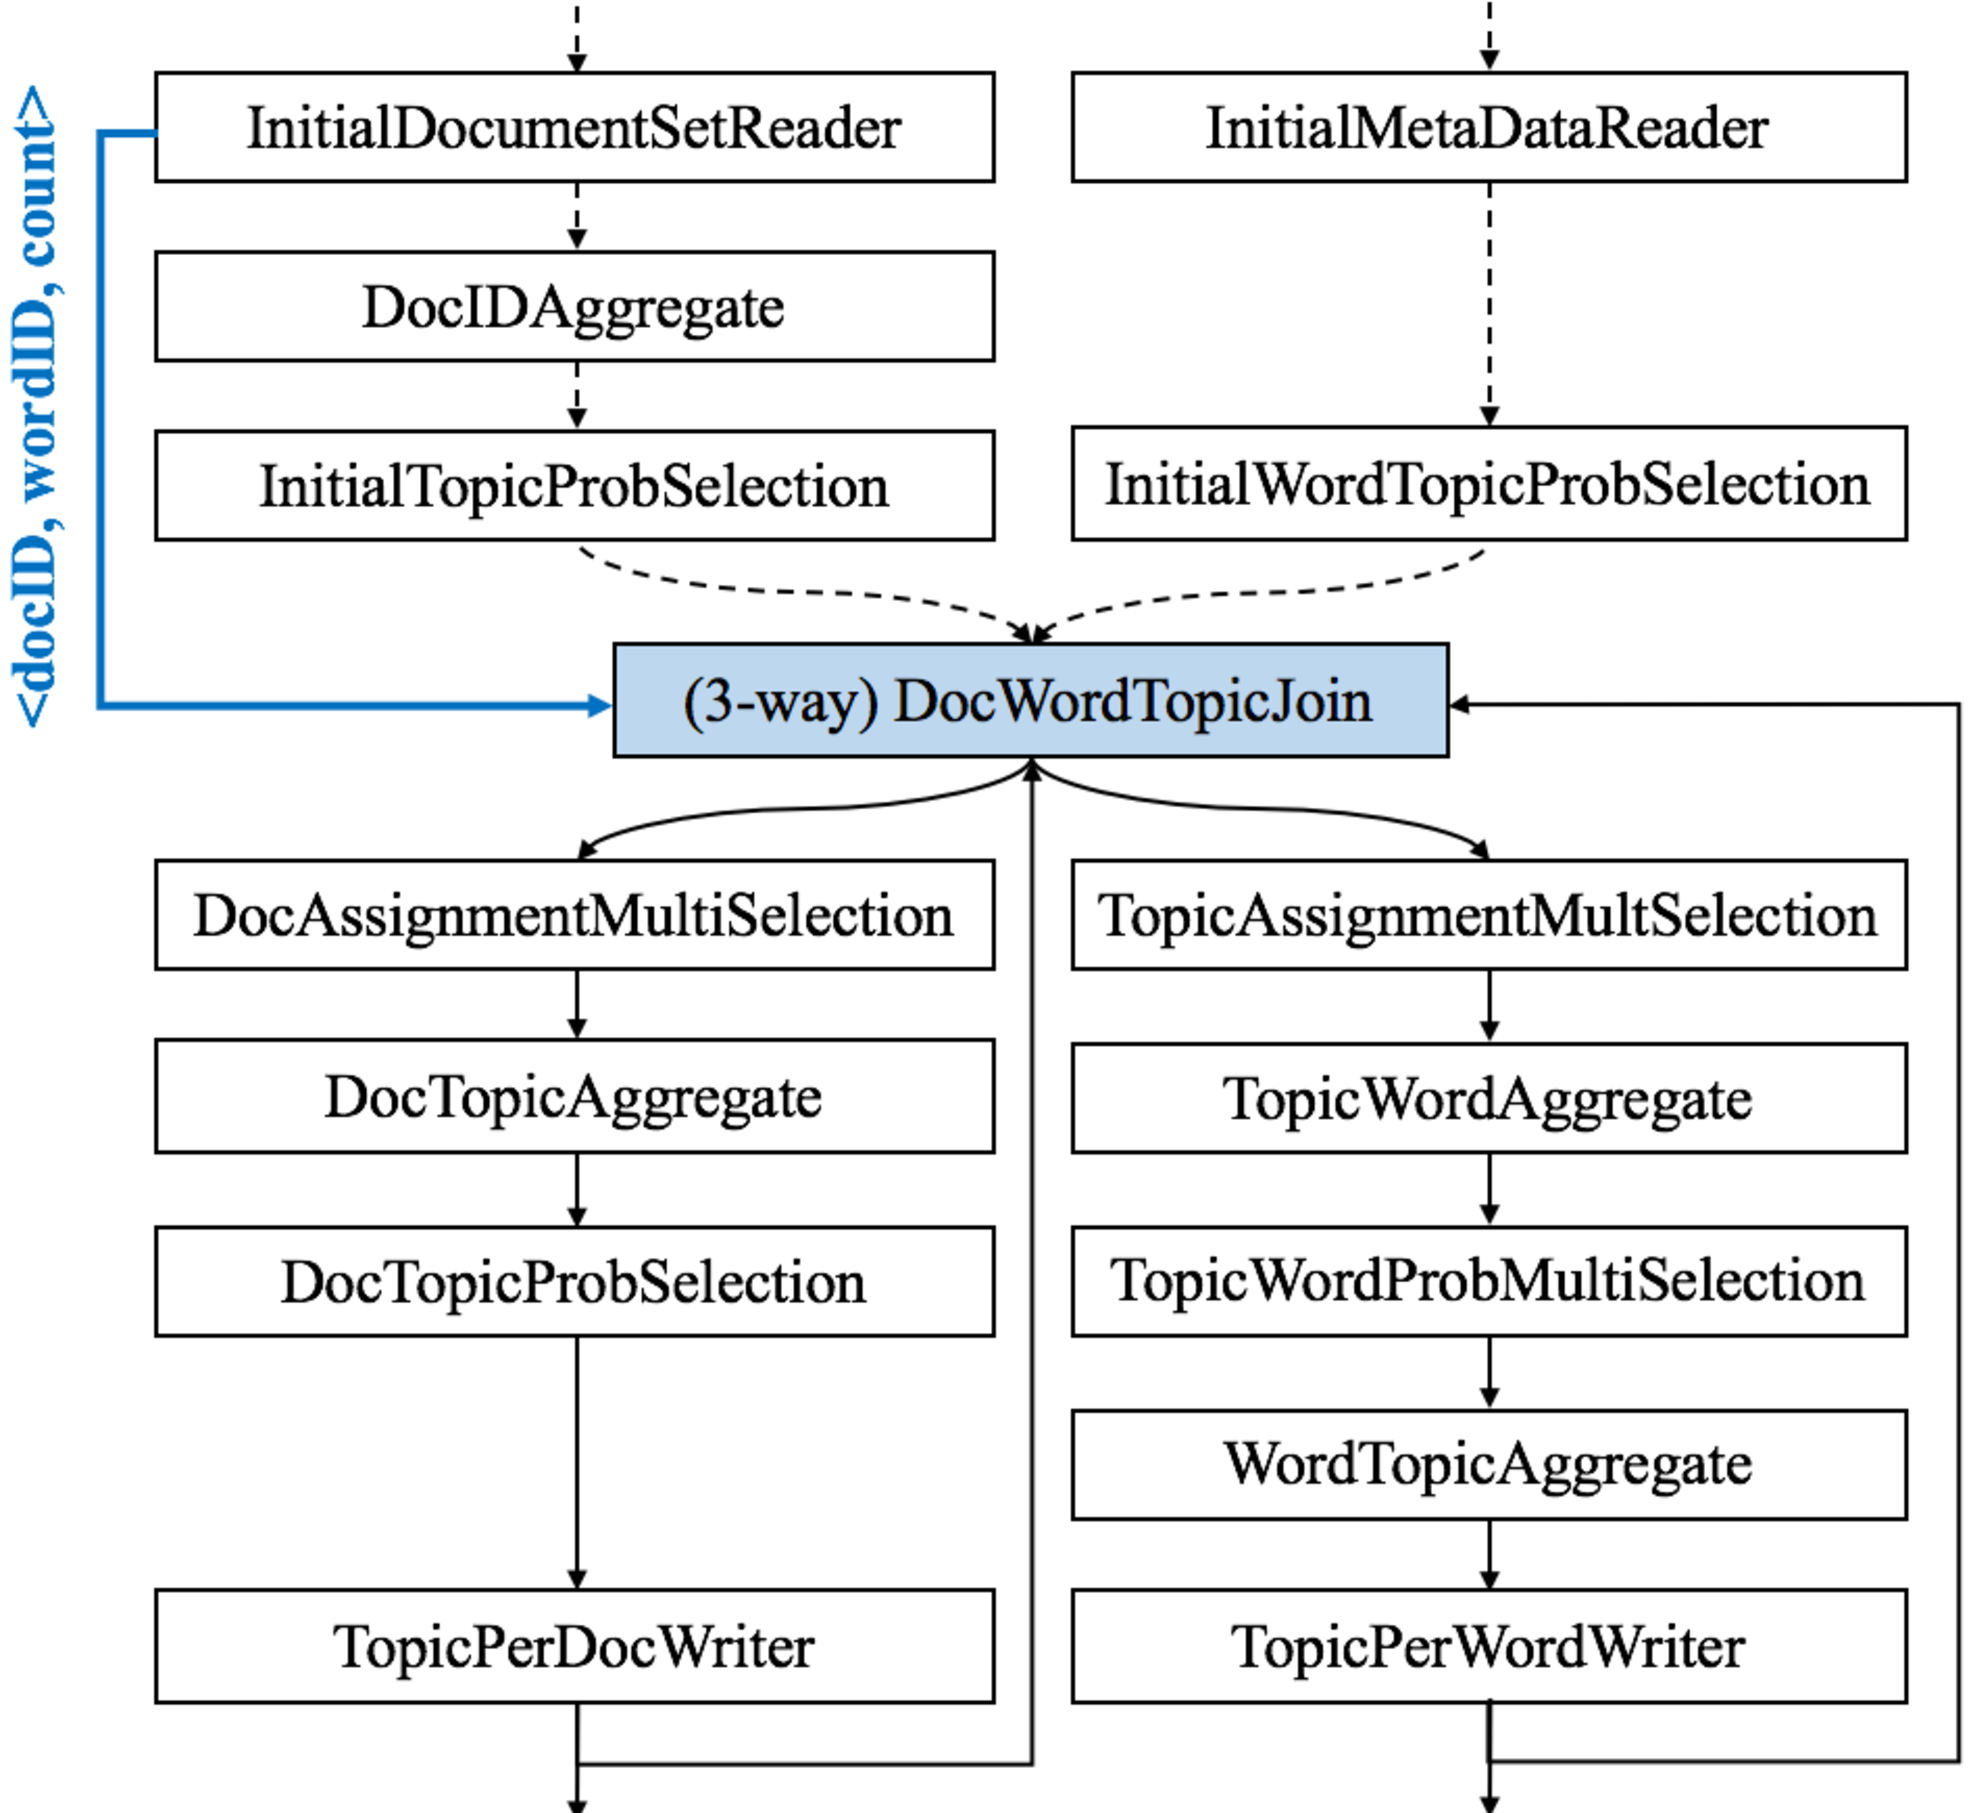
\includegraphics[width=0.5\textwidth]{lda-query-graph.pdf}
  \caption{\label{fig:lda-query-graph} LDA's query graph. Computation
    connected by dash lines will only run once for
    initialization. Computation connected by solid lines will run iteratively.}
\end{figure}


\vspace{5pt}
The LDA offering in the Spark MLLib is based on Expectation
Maximization and Online Variational Bayes, which is very different
with our implementation. Therefore we asked a Spark expert to carefully implement an algorithmatically
equivalent LDA in Spark using combined RDD and DataSet        
APIs. 

For GMM and KMeans, instead of implementing
our own Spark applications, we chose to use Spark MLLib
implementations of those two workloads, and we implement those two
workloads in PC to be consistent with their Spark equivalents.

\vspace{5pt}
\noindent
\texttt { GMM.} A Gaussian mixture model (GMM) can be used to model data points that come
from one of $K$ clusters, and data points within the same cluster
can be modeled by a Gaussian distribution. So the $k$-th Gaussian
distribution is parameterized by a mean vector $\mu_k$ and a covariance
matrix $\sum_k$, and has a probability distribution $\pi_k$.

For this experiment, we
implemented GMM using the Expectation Maximization (EM) algorithm to be
consistent with the GMM algorithm implemented in Spark Mllib. EM is an
iterative optimization technique that consists of two steps in each
iteration: an estimation step to determine ``responsibility'' score
for assigning each data point to each Gaussian $k$ using the current model; and a maximization step to
update the model parameters using the new ``responsibility'' score. A complex
aggregation will run in each iteration to complete the two steps. The algorithm repeats
the two steps until log likelihood or parameters converges. 

\vspace{5pt}
\noindent
\texttt {KMeans.} We developed a KMeans implementation on PC, which
is equivalent with the KMeans implementation in Spark MLLib. Spark
MLLib KMeans implementation has two initialization approach: KMeans++
and random initialization using sampling. For both experiments, we use
random initialization by sampling $K$ data points as initial
cluster centroids. For initialization, both implementations also compute $L^2$ norm for each data
point, and transform each data point into a new form with $L^2$ norm value
associated. 

Then in each iteration, each data point finds the closest cluster
of which the centroid has the closest distance with that data point, and assigns the closest
cluster label to itself. When computing the distance of a data point to a
centroid, a lower bound based on $\|a - b\| \geq |\|a\| - \|b\||$ is
first computed to avoid unnecessary distance computation. Then an aggregation is run to update centroids
based on computed new labels. Iteration repeats until centroids
converge.


\subsubsection {Experiments}

On the 10-worker cluster aforementioned, we run experiments for LDA,
GMM and KMeans on both PC and Spark 2.1.0 platforms. 

For LDA,  we
create a synthetic document database with 2.5 million documents from
20 newsgroups data set by concatenate postings
end-on-end~\cite{jermaineExperimental}. We also use a dictionary size
of 20000 words and a model size of 100 topics. For GMM, we generate
random data for three test cases: $10^7$ data
points with 100 dimenisons, and $10^6$ data points with 300 and 500
dimensions, respectively. For each test case, same random data is used
for comparing PC and Spark performance. For KMeans, we
generate randome data for $10^9$ data
points with 10 dimenisons, $10^8$ data points with 100 dimensions,  and $10^7$
data points with 1000
dimensions. Similar with GMM, for each test case, same random data is used on both PC and
Spark platforms.

For each experiment, we carefully tune PC page sizes, buffer pool
size, thread number, and Spark
partition size, executor heap size and core number to make sure all
resources are fully utilized.




\subsubsection {Results}

LDA Results (per iteration) are illustrated in Tab.~\ref{fig:LDA}:

\begin{table}[h!]
\begin{center}
\begin{tabular}{|c||c|c|c|c|c|c|}
\hline
PlinyCompute & \makecell{Spark 1: \\vanilla} & \makecell{Spark 2: also with \\join hint} & \makecell{Spark 3: also with \\forced persist} & \makecell{Spark 3: also hand-\\coded multinomial} \\
\hline
02:05 & 50:20 & 17:30 & 09:26 & 05:26 \\
\hline
\end{tabular}
\caption{PlinyCompute vs. Spark for LDA. Times in MM:SS, averaged over five iterations.}
\label{fig:LDA}
\end{center}
\end{table}
\vspace{-10pt}
While Spark performed well, the 
amount of work required to arrive at a good solution 
was significant, representing about a week of tuning.  First, among other things, our Spark expert had to force a 
broadcast join.  Then, it was necessary to force Spark to
persist the result of one of the joins for later use.  Finally, it was necessary to hand-code a 
Multinomial sampler to obtain an implementation that was competitive with PC.
This illustrates the advantage of PC's declarative approach: decisions such as broadcast vs. full hash
join as well as which intermediate results to materialize are
automated. 

\vspace{5pt}
For GMM, as illustrated in Tab.~\ref{fig:Gmm}, PC achieved a 
$3\times$ speedup compared with Spark MLLib for all cases.

\begin{table}[h!]
\begin{center}
\begin{tabular}{|c||c|c|c||}
\hline
Dimensionality & $100$ & $300$ & $500$ \\
Number of points & $10^7$ & $10^6$ & $10^6$ \\
\hline
\hline
PlinyCompute &00:30 & 00:38 & 1:42 \\
Spark \texttt{mllib} &1:41  &1:54 &5:05 \\
\hline
\end{tabular}
\caption{PlinyCompute vs. Spark for GMM. Times in MM:SS, averaged over five iterations.}
\label{fig:Gmm}
\end{center}
\end{table}



\vspace{5pt}
As illustrated in Tab.~\ref{fig:KMeans}, for KMeans workload, PC achieved a $2\times$ to
$4\times$ speedup compared with Spark MLLib. 

\begin{table}[h!]
\begin{center}
\begin{tabular}{|c||c|c|c||c|c|c||}
\hline
& \multicolumn{3}{c||}{Initialization Latency} & \multicolumn{3}{c||}{Average
                                         Iteration Latency} \\
\hline
Dimensionality & $10$ & $100$ & $1000$ & $10$ & $100$ & $1000$\\
Number of points & $10^9$ & $10^8$ & $10^7$ & $10^9$ & $10^8$ & $10^7$\\
\hline
PlinyCompute &3:59 & 1:12 & 00:57 &00:37 & 00:09 & 00:06\\
Spark \texttt{mllib} &9:06  &4:18 &3:20 &01:02 & 00:28 & 00:23\\
\hline
\end{tabular}
\caption{PlinyCompute vs. Spark for KMeans. Times in MM:SS, averaged over five iterations.}
\label{fig:KMeans}
\end{center}
\end{table}


\subsubsection{Discussions}
For iterative and complex machine learning
benchmarks, compared with equivalent and carefully tuned implementations on the latest
Spark platform, PC still achieved $2 \times$ to $4 \times$
speedup. On one side this demonstrated PC's utility in handling
complex and iterative computations. On the other side, we've found that due to the complexity in mathematical and statistical
computations in those workloads, in many cases performance comparison is reduced to comparisons of
language efficiency and compiler supports. So it also indicates that PC has a
potential to achieve even larger performance gain by better
synergizing with C++ compiler and link-time optimizing tool chains.



\subsection{Summary}

\begin{table}[h!]
\begin{center}
\begin{tabular}{|c|c|c|}
\hline
Applications & LOC on PlinyCompute & LOC on Spark\\
\hline
Linear Algebra Package &3505& 3130 (scala)\\
TPC-H \texttt{Customer}s per \texttt{Supplier}&929 &953 (Java)\\
TPC-H top-$k$ Jaccard &793 & 966 (Java)\\
LDA &1038  &314 (Scala)\\
GMM&932 & 474 (Scala with Breeze)\\
KMeans &695  &670 (Scala)\\
\hline
\end{tabular}
\caption{PlinyCompute vs. Spark: Lines of Source Code Comparison.}
\label{fig:LOC}
\end{center}
\end{table}


